\documentclass[border=0.2cm]{standalone}
 
\usepackage{tikz}
 
\begin{document}
 
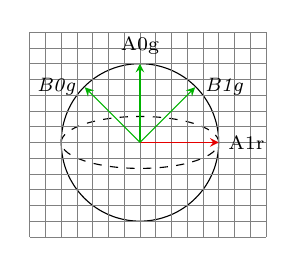
\begin{tikzpicture}
	\draw (0,0) circle (1cm);
	\draw [thin,dashed](0,0) ellipse (1cm and 0.33cm);
	\draw[step=0.2cm,gray,very thin] (-1.4,-1.2) grid (1.6,1.4);
	
	\draw [-stealth,black!10!red](0,0) -- (1,0) node[right,black]{\scriptsize A1r};
	\draw [-stealth,black!30!green](0,0) -- (.7,.7) node[right,black]{\scriptsize\itshape B1g};
	\draw [-stealth,black!30!green](0,0) -- (-.7,.7) node[left,black]{\scriptsize\itshape  B0g};
	\draw [-stealth, black!30!green](0,0) -- (0,1) node[above,black]{\scriptsize A0g};
\end{tikzpicture}
 
\end{document}

